\chapter{Related work}
\label{chapters:related-work}

This tool follows previous research that was carried out by the \textit{XML and Web Engineering Research Group} (XRG) at the Faculty of Mathematics and Physics of the Charles University in the years 2012 to 2015.

The following section introduces the research's core concepts that will be analyzed and used in the thesis, followed by the section on similar work in the research area.

\section{Previous research}

In 2012 XRG formalized a novel approach\footnote{The work builds on previous work of the same authors where they introduced the XSEM model \cite{necasky2007xsem}, which has later been a subject of their study.} to modeling XML schemas \cite{necasky2012conceptual} for a particular domain ontology by integrating Model-Driven Development (specifically Model-Driven Architecture) techniques to separate a conceptual model describing the domain ontology and a structural model which described the concrete XML schema.

Model-Driven Architecture is a software engineering technique that abstracts development into three viewpoints: CIM as the \textit{Computation-independent Model}, PIM as the \textit{Platform-independent model} and PSM as the \textit{Platform-specific model}.

XRG used only the last two layers of the architecture. PIM represents the domain ontology in UML-like notation\footnote{Formal definition of PIM and PSM levels is in chapter \ref{chapters:formal-background}.}, as it is independent of the platform as XML. PSM as a platform-specific then represents the given schema in their own designed grammar, which was translated into a final schema, such as XSD.

\begin{figure}[h]\centering
    \begin{tikzpicture}[
        squarednode/.style={rectangle, draw=blue!60, fill=blue!5, very thick, minimum size=5mm},
    ]
        %Nodes
        \node[squarednode] (pim) at (0,0) {PIM schema};
        \node[squarednode] (psm1) at (-2.5,-1.5) {PSM schema 1};
        \node (psmDot) at (0,-1.5) {...};
        \node[squarednode] (psmN) at (2.5,-1.5) {PSM schema N};

        \node[squarednode] (schema1) at (-2.5,-3) {XML schema 1};
        \node (psmDot) at (0,-3) {...};
        \node[squarednode] (schemaN) at (2.5,-3) {XML schema N};

        \node[squarednode,cascaded] (q1) at (-1.5,-4.5) {XML queries};
        \node (psmDot) at (1,-4.5) {...};
        \node[squarednode,cascaded] (qN) at (3.5,-4.5) {XML queries};

        \node[squarednode,cascaded] (document1) at (-2.5,-6) {XML documents};
        \node (psmDot) at (0,-6) {...};
        \node[squarednode,cascaded] (documentN) at (2.5,-6) {XML documents};

        \node (psm_t)[text width=4cm,align=right] at (-7,0) {{Platform-specific level:}};
        \node (pim_t)[text width=4cm,align=right] at (-7,-1.5) {{Platform-independent level:}};
        \node (schema_t)[text width=4cm,align=right] at (-7,-3) {{Schema/Logical level:}};
        \node (ext_t)[text width=4cm,align=right] at (-7,-4.5) {{Operational level:}};
        \node (ext_t)[text width=4cm,align=right] at (-7,-6) {{Extensional level:}};

        %Lines
        \draw[-latex] (psm1) -- (pim);
        \draw[-latex] (psmN) -- (pim);
        \begin{scope}[transform canvas={xshift=-2em}]
            \draw[-latex] (document1) -- (schema1); % node[fill=white]{conforms}
            \draw[-latex] (documentN) -- (schemaN); % node[fill=white]{conforms}
        \end{scope}
        \draw[-latex] (schema1) -- (psm1);
        \draw[-latex] (schemaN) -- (psmN);
        \draw[-latex] (q1) -- (schema1);
        \draw[-latex] (qN) -- (schemaN);

        % separators
        \foreach \x in {0,...,3}{
            \draw [dotted] (-9,-0.75-1.5*\x) -- (5,-0.75-1.5*\x);
        }
    \end{tikzpicture}
    \caption{The five-level framework proposed by XRG in \cite{necasky2012conceptual}. A shared PIM layer with a conceptual model is used by multiple PSMs, where schemas are defined in their own grammar. The grammar is then translated into schemas that conform to XML documents.}
\end{figure}

The major benefit of the strategy presented is a shared conceptual model between various XML schemas, as other works at that time had a conceptual model for every schema. This was not practical as usually multiple schemas are applied in a single software. Authors have also formalized the model and have proven that their approach is correct. That means that (i) every conceptual schema models XML schema, (ii) their translation algorithm from the internal model to schema respects introduced rules and is reversible, and (iii) their normalization and optimization algorithms produce semantically same schema.

\begin{figure}[h!]
    \centering
    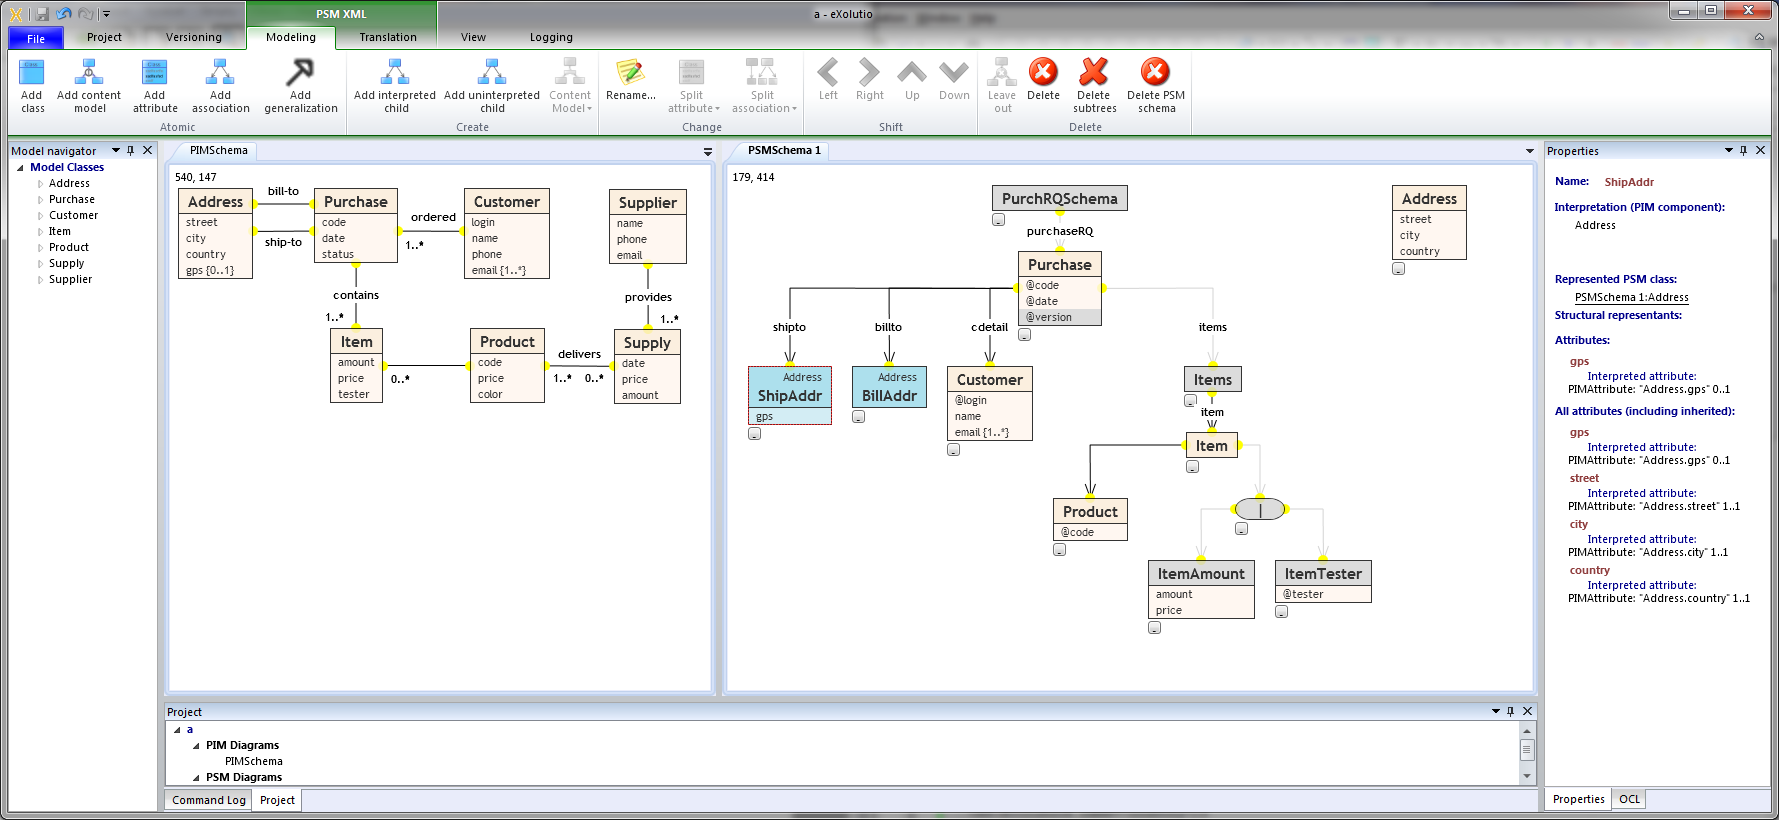
\includegraphics[width=0.8\textwidth]{img/exolutio.png}
    \caption{Preview of the eXolutio tool. The left panel shows the PIM model as a UML class diagram, while the right panel represents a PSM schema in a tree-like structure that can be converted to an XML schema.}
    \label{fig:exolutio}
\end{figure}

\subsection{Evolution of schemas}

The focus of XRG was also directed to the evolution \cite{nevcasky2012evolution} of their proposed model to minimize the work of the data designer. As already stated in the introduction of the thesis, changes may be inevitable (either from the user requirements or from the surrounding environment) in large and complex systems, and propagating even a tiny change from the domain ontology to all affected schemas is time-consuming and error-prone.

They proposed, formalized, and later implemented a solution in restricting the changes in PIM and PSM models to only atomic operations - simple changes in the model, such as \textit{creating a new class}, \textit{updating a name of association} or \textit{removing an attribute}. Those operations are not intended to be used by the user directly but are simple enough to be formally defined and mapped to the corresponding operations in the level below. The proposed mapping is then used to propagate changes in the model to the schema level, more precisely from PSM to PIM, which is then translated to the schema level. They implemented only top-down propagation of changes as the propagation from XML documents is usually not meaningful (but theoretically possible).

\subsection{Implementation}

Their result were implemented in two tools \textit{XCase} \cite{xcase} and \textit{eXolutio} \cite{exolutio}. The former one was simpler, focused only on modeling. The latter then supported schema evolution as described in the previous section. Tools let users define the ontology from which the schemas and operations were derived for XML documents.

\section{OSLO}

OSLO\footnote{\url{https://joinup.ec.europa.eu/collection/oslo-open-standards-linked-organisations-0/about}} - Open Standards for Linked Organisations is an initiative that originated in Flanders, Dutch-speaking northern portion of Belgium, to promote the use of technical standards for the data exchange between various organizations, government, and a local government. The goal of OSLO is to maintain and create the standards through the open process (hence everyone can intervene), keep the rules respected, provide a publication platform and support the adoption of the standards. So far, OSLO contains over 18 different domains consisting definitions from 107 organizations.

The initiative developed a toolchain to ease the process of publication of the standards. The standards are modeled in \textit{Enterprise Architect UML} software and then converted into an RDF representation with their tool\footnote{\url{https://github.com/Informatievlaanderen/OSLO-EA-to-RDF}}. The next tool then generates artifacts (resulting files) that are automatically published on one centralized server \url{https://data.vlaanderen.be/ns}. The artifacts contain HTML documentation, RDF vocabulary, SHACL templates for validation of RDF, and a JSON-LD context for developers that prefer JSON formats. Their toolchain uses the GitHub platform for storing their standards and triggering the rest of the toolchain. They also provide tools for organizations to validate their data against the standards to check that data are machine-readable without errors.

OSLO also focuses on the interoperability of services that provide those data so that every service has a generic hyper-media-driven API.

\medskip

Compared to our approach, OSLO's primary focus is on the interoperability of public services and their data in LOD format. Their goal is to provide a set of tools to create and later validate public services effectively. Our approach is to design a general tool (hence it can be used for any related purpose, such as software development process) for services that use non-RDF formats, such as CSV or XML files, and rather provide tools to convert them to linked data format.

As noted in the introduction chapter, we also focus on the public sector. Yet, our tool is not as advanced as theirs to provide features such as (i) automatic publishing of the standards or (ii) web tools to validate organizations-data against them. Nevertheless, we may take a similar route for the open data publication process in the future.

\section{LinkML}

LinkML is a general-purpose language using YAML for modeling schemas that can be converted to various formats such as JSON, CSV, RDF, or Python Dataclasses. It also generates human-readable documentation and can validate the data in different formats.

The core concepts in their model are classes and slots, which are properties of classes. Classes then support inheritance. The model supports many options for the data types, cardinalities, regular expression patterns, and other constraints.


\begin{figure}[h!]\centering
    \begin{Verbatim}[commandchars=\\\{\}]
classes:
  Person:
    attributes:
      id:
        identifier: true
      full_name:
        required: true
        description:
          name of the person
      aliases:
        multivalued: true
        description:
          other names for the person
      phone:
        pattern: "^[\textbackslash{}\textbackslash{}d\textbackslash{}\textbackslash{}(\textbackslash{}\textbackslash{})\textbackslash{}\textbackslash{}-]+$"
      age:
        range: integer
        minimum_value: 0
        maximum_value: 200
    \end{Verbatim}
    \caption{Example of part of the YAML configuration file for LinkML.}
\end{figure}


\section{Similar work}

\td{
    \begin{itemize}
        \item Google Scholar docela něco vrací na "model driven transformation cim pim data schema".
        \item Dále pak jsem našel možná relevantní - https://link.springer.com/article/10.1007/s10270-021-00905-x. K článkům byste se měl z univerzitní sítě dostat zdarma.
    \end{itemize}
}